\section{Higher Order Constant Coefficient Homogeneous Equations}

\noindent
If $a_0$, $a_1$, \dots, $a_n$ are constants and $a_0\ne0$, then
$$
a_0y^{(n)}+a_1y^{(n-1)}+\cdots+a_ny=F(x)
$$
is said to be a {\color{blue}\it constant coefficient equation\/}.
In this section we consider the homogeneous constant coefficient
equation
\begin{equation} \label{eq:9.2.1}
a_0y^{(n)}+a_1y^{(n-1)}+\cdots+a_ny=0.
\end{equation}
Since \eqref{eq:9.2.1} is normal on $(-\infty,\infty)$, the theorems in
Section~9.1 all apply with $(a,b)=(-\infty,\infty)$.

As in Section~5.2, we call
\begin{equation} \label{eq:9.2.2}
p(r)=a_0r^n+a_1r^{n-1}+\cdots+a_n
\end{equation}
the {\color{blue}\it characteristic polynomial\/} of \eqref{eq:9.2.1}. We saw in
Section~5.2 that when $n=2$ the solutions of \eqref{eq:9.2.1} are
determined by the zeros of the characteristic polynomial. This is also
true when $n>2$, but the situation is more complicated in this case.
Consequently, we take a different approach here than in
Section~5.2.

If $k$ is a positive integer, let $D^k$ stand
for the $k$-th derivative operator;   that is
$$
D^ky=y^{(k)}.
$$
If
$$
q(r)=b_0r^m+b_1r^{m-1}+\cdots+b_m
$$
is an arbitrary polynomial,  define the operator
$$
q(D)=b_0D^m+b_1D^{m-1}+\cdots+b_m
$$
such that
$$
q(D)y=(b_0D^m+b_1D^{m-1}+\cdots+b_m)y=b_0y^{(m)}+b_1y^{(m-1)}+\cdots+
b_my
$$
whenever $y$ is a function with $m$ derivatives. We call $q(D)$
a {\color{blue}\it polynomial\/}  operator.

With $p$ as in \eqref{eq:9.2.2},
$$
p(D)=a_0D^n+a_1D^{n-1}+\cdots+a_n,
$$
so \eqref{eq:9.2.1} can be written as $p(D)y=0$.  If $r$ is a constant
then
\begin{eqnarray*}
p(D)e^{rx}&=&\left(a_0D^ne^{rx}+a_1D^{n-1}e^{rx}+\cdots+a_ne^{rx}\right)\\
&=&(a_0r^n+a_1r^{n-1}+\cdots+a_n)e^{rx};
\end{eqnarray*}
that is
$$
p(D)(e^{rx})=p(r)e^{rx}.
$$
This shows that $y=e^{rx}$ is a solution of \eqref{eq:9.2.1}
if $p(r)=0$.
In the simplest case, where $p$ has $n$ distinct real zeros
$r_1$, $r_2$,\dots, $r_n$, this argument yields $n$ solutions
$$
y_1=e^{r_1x},\quad y_2=e^{r_2x},\dots,\quad y_n=e^{r_nx}.
$$
It can be shown (Exercise~\ref{exer:9.2.39}) that the Wronskian of
$\{e^{r_1x},e^{r_2x},\dots,e^{r_nx}\}$ is nonzero if
$r_1$, $r_2$, \dots, $r_n$ are distinct; hence,
$\{e^{r_1x},e^{r_2x},\dots,e^{r_nx}\}$
is a fundamental set of solutions of $p(D)y=0$ in this case.

\begin{example}\label{example:9.2.1} \rm  \mbox{}\newline
\begin{alist}
\item %(a)
Find the general solution of
\begin{equation} \label{eq:9.2.3}
y'''-6y''+11y'-6y=0.
\end{equation}
\item %(b)
Solve the initial value problem
\begin{equation} \label{eq:9.2.4}
y'''-6y''+11y'-6y=0, \quad  y(0)=4,\quad y'(0)=5,\quad y''(0)=9.
\end{equation}
\end{alist}
\end{example}

\solution The characteristic polynomial of
\eqref{eq:9.2.3} is
$$
p(r)=r^3-6r^2+11r-6=(r-1)(r-2)(r-3).
$$
Therefore $\{e^x,e^{2x},e^{3x}\}$ is a set of solutions of
\eqref{eq:9.2.3}. It is a fundamental set, since its Wronskian is
$$
W(x)=\left|\begin{array}{rrr}e^x&e^{2x}&e^{3x}\\e^x&2e^{2x}&
3e^{3x}\\e^x&4e^{2x}&9e^{3x}\end{array}\right|=
e^{6x}\left|\begin{array}{rrr}1&1&1\\1&2&
3\\1&4&9\end{array}\right|=2e^{6x}\ne0.
$$
Therefore the general solution of \eqref{eq:9.2.3} is
\begin{equation} \label{eq:9.2.5}
y=c_1e^{x}+c_2e^{2x}+c_3e^{3x}.
\end{equation}

\solutionpart{b} We must determine $c_1$, $c_2$ and $c_3$ in
\eqref{eq:9.2.5}
so that $y$ satisfies the initial conditions in \eqref{eq:9.2.4}.
Differentiating \eqref{eq:9.2.5} twice yields
\begin{equation} \label{eq:9.2.6}
\begin{array}{rcl}
y'&=&c_1e^{x}+2c_2e^{2x}+3c_3e^{3x}\\
y''&=&c_1e^{x}+4c_2e^{2x}+9c_3e^{3x}.
\end{array}
\end{equation}
Setting $x=0$ in \eqref{eq:9.2.5} and \eqref{eq:9.2.6}  and imposing the
initial conditions yields
$$\begin{array}{rcl}
c_1+\phantom{2}c_2+\phantom{3}c_3&=&4\\
c_1+2c_2+3c_3&=&5\\
c_1+4c_2+9c_3&=&9.
\end{array}$$
The solution of this system is $c_1=4$, $c_2=-1$, $c_3=1$. Therefore the
solution of \eqref{eq:9.2.4} is
 $$
y=4e^x-e^{2x}+e^{3x}
$$
(Figure~\ref{figure:9.2.1}).
\bbox

\begin{figure}[tbp]
  \centering\color{blue}
  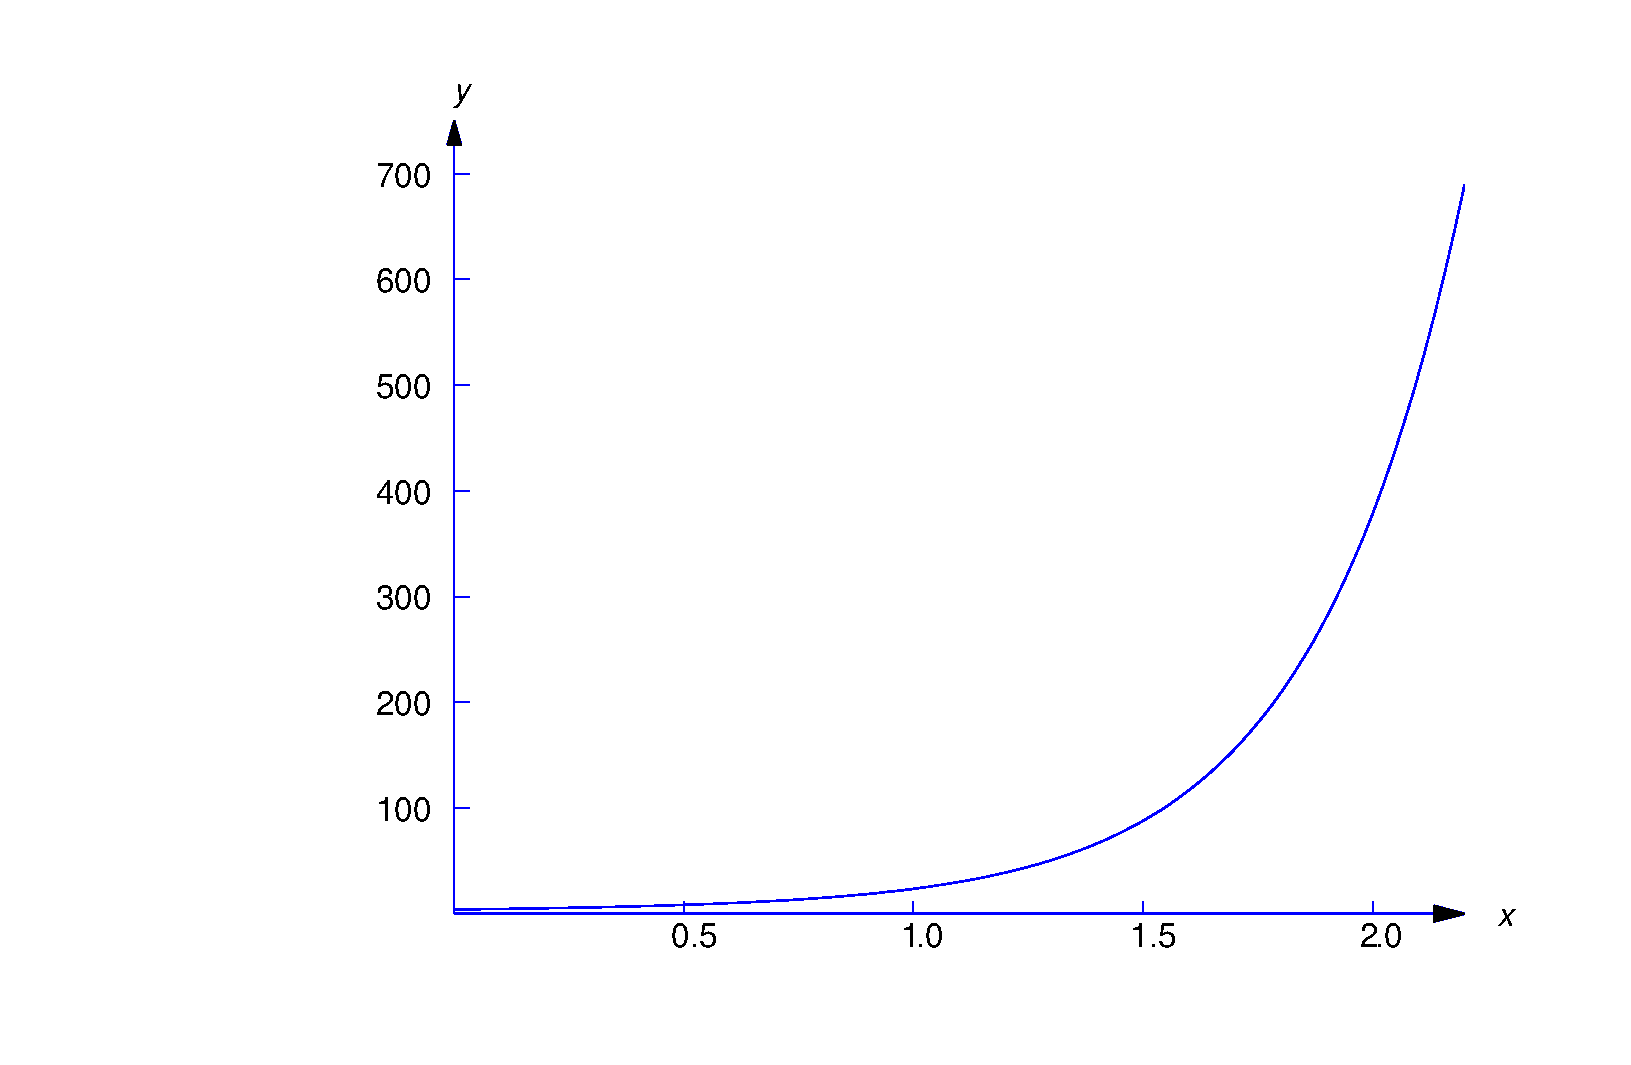
\includegraphics[bb=-78 148 689 643,width=5.67in,height=3.66in,keepaspectratio]{fig090201}
\caption{$y=4e^x-e^{2x}+e^{3x}$}
  \label{figure:9.2.1}
\end{figure}

Now we consider the case where the characteristic polynomial
\eqref{eq:9.2.2} does not have $n$ distinct real zeros. For this purpose
it is useful to define what we mean by a factorization of a polynomial
operator. We begin with an example.

\begin{example}\label{example:9.2.2} \rm
Consider the polynomial
$$
p(r)=r^3-r^2+r-1
$$
and the associated polynomial operator
$$
p(D)=D^3-D^2+D-1.
$$
Since $p(r)$ can be factored as
$$
p(r)=(r-1)(r^2+1)=(r^2+1)(r-1),
$$
it's reasonable to expect that p(D) can be factored as
\begin{equation} \label{eq:9.2.7}
p(D)=(D-1)(D^2+1)=(D^2+1)(D-1).
\end{equation}
However, before we can make this assertion we must {\color{blue}\it define\/}
 what we mean by saying that two operators are equal, and what we mean
by the products of operators in \eqref{eq:9.2.7}. We say that two
operators are equal if they apply to the same functions and always
produce the same result. The definitions of the products in
\eqref{eq:9.2.7} is this: if $y$ is any three-times differentiable
function then
\begin{alist}
\item % (a)
$(D-1)(D^2+1)y$
is the function obtained by first applying $D^2+1$ to $y$ and then
applying $D-1$ to the resulting function
\item % (b)
$(D^2+1)(D-1)y$
is the function obtained by first applying $D-1$ to $y$ and then
applying $D^2+1$ to the resulting function.
\end{alist}
From \part{a},
\begin{equation} \label{eq:9.2.8}
\begin{array}{rcl}
(D-1)(D^2+1)y&=&(D-1)[(D^2+1)y]\\
&=&(D-1)(y''+y)=D(y''+y)-(y''+y)\\&=&(y'''+y')-(y''+y)\\
&=&y'''-y''+y'-y=(D^3-D^2+D-1)y.
\end{array}
\end{equation}
This implies that
$$
(D-1)(D^2+1)=(D^3-D^2+D-1).
$$
From \part{b},
\begin{equation} \label{eq:9.2.9}
\begin{array}{rcl}
(D^2+1)(D-1)y&=&(D^2+1)[(D-1)y]\\
&=&(D^2+1)(y'-y)=D^2(y'-y)+(y'-y)\\&=&(y'''-y'')+(y'-y)\\
&=&y'''-y''+y'-y=(D^3-D^2+D-1)y,
\end{array}
\end{equation}
$$
(D^2+1)(D-1)=(D^3-D^2+D-1),
$$
which completes the justification of \eqref{eq:9.2.7}.
\end{example}

\begin{example}\label{example:9.2.3} \rm
Use the result of Example~\ref{example:9.2.2} to find the general
solution of
\begin{equation} \label{eq:9.2.10}
y'''-y''+y'-y=0.
\end{equation}
\end{example}

\solution
From \eqref{eq:9.2.8}, we can rewrite \eqref{eq:9.2.10} as
$$
(D-1)(D^2+1)y=0,
$$
which implies that any solution of $(D^2+1)y=0$ is a solution of
\eqref{eq:9.2.10}. Therefore $y_1=\cos x$ and $y_2=\sin x$ are solutions
of \eqref{eq:9.2.10}.

From \eqref{eq:9.2.9}, we can rewrite \eqref{eq:9.2.10} as
$$
(D^2+1)(D-1)y=0,
$$
which implies that any solution of $(D-1)y=0$ is a solution of
\eqref{eq:9.2.10}. Therefore $y_3=e^x$ is solution of \eqref{eq:9.2.10}.

The Wronskian of $\{e^x,\cos x,\sin x\}$ is
$$
W(x)=\left|\begin{array}{rrr}\cos x&\sin x&e^x\\-\sin x&\cos x&e^x\\
-\cos x&-\sin x&e^x\end{array}\right|.
$$
Since
$$
W(0)=\left|\begin{array}{rrr}1&0&1\\0&1&1\\
-1&0&1\end{array}\right|=2,
$$
 $\{\cos x,\sin x,e^x\}$ is linearly independent
and
$$
y=c_1\cos x+c_2\sin x+c_3e^x
$$
is the general solution of \eqref{eq:9.2.10}.

\begin{example}\label{example:9.2.4} \rm
Find the general solution of
\begin{equation} \label{eq:9.2.11}
y^{(4)}-16y=0.
\end{equation}
\end{example}

\solution  The characteristic polynomial of
\eqref{eq:9.2.11} is
$$
p(r)=r^4-16=(r^2-4)(r^2+4)=(r-2)(r+2)(r^2+4).
$$
By arguments similar to those used in Examples~\ref{example:9.2.2} and
\ref{example:9.2.3}, it can be shown that \eqref{eq:9.2.11} can be written
as
$$
(D^2+4)(D+2)(D-2)y=0
$$
or
$$
(D^2+4)(D-2)(D+2)y=0
$$
or
$$
(D-2)(D+2)(D^2+4)y=0.
$$
Therefore $y$  is a solution of \eqref{eq:9.2.11} if it's a solution
of any  of the three  equations
$$
 (D-2)y=0,\quad (D+2)y=0, \quad(D^2+4)y=0.
$$
Hence, $\{e^{2x},e^{-2x},\cos2x,\sin2x\}$ is a set of solutions of
\eqref{eq:9.2.11}. The Wronskian of this set is
$$
W(x)=\left|\begin{array}{rrrr}
e^{2x}&e^{-2x}&\cos2x&\sin2x\\
2e^{2x}&-2e^{-2x}&-2\sin2x&2\cos2x\\
4e^{2x}&4e^{-2x}&-4\cos2x&-4\sin2x\\
8e^{2x}&-8e^{-2x}&8\sin2x&-8\cos2x\\
\end{array}\right|.
$$
Since
$$
W(0)=\left|\begin{array}{rrrr}
1&1&1&0\\
2&-2&0&2\\
4&4&-4&0\\
8&-8&0&-8\\
\end{array}\right|=-512,
$$
 $\{e^{2x},e^{-2x},\cos2x,\sin2x\}$ is linearly independent,
and
$$
y_1=c_1e^{2x}+c_2e^{-2x}+c_3\cos2x+c_4\sin2x
$$
is   the general solution of \eqref{eq:9.2.11}.

It is known from algebra that every polynomial
$$
p(r)=a_0r^n+a_1r^{n-1}+\cdots+a_n
$$
with real coefficients can be factored as
$$
p(r)=a_0p_1(r)p_2(r)\cdots p_k(r),
$$
where no pair of the polynomials $p_1$, $p_2$, \dots, $p_k$  has a common
factor and each  is either of the form
\begin{equation} \label{eq:9.2.12}
p_j(r)=(r-r_j)^{m_j},
\end{equation}
where $r_j$ is real and $m_j$ is a positive integer, or
\begin{equation} \label{eq:9.2.13}
p_j(r)=\left[(r-\lambda_j)^2+\omega_j^2\right]^{m_j},
\end{equation}
where $\lambda_j$ and $\omega_j$ are real, $\omega_j\ne0$, and $m_j$
is a positive integer. If \eqref{eq:9.2.12} holds then $r_j$ is a real
zero of $p$, while if \eqref{eq:9.2.13} holds then $\lambda+i\omega$
and $\lambda-i\omega$ are complex conjugate zeros of $p$. In either
case, $m_j$ is the {\color{blue}\it multiplicity\/} of the zero(s).

By arguments similar to those used in our examples, it can be shown
that
\begin{equation} \label{eq:9.2.14}
p(D)=a_0p_1(D)p_2(D)\cdots p_k(D)
\end{equation}
and that the order of the factors on the right can be chosen
arbitrarily. Therefore, if $p_j(D)y=0$ for some $j$ then
$p(D)y=0$. To see this, we simply rewrite \eqref{eq:9.2.14} so that
$p_j(D)$ is applied first. Therefore the problem of finding solutions
of $p(D)y=0$ with $p$ as in \eqref{eq:9.2.14} reduces to finding solutions
of each of these equations
$$
p_j(D)y=0,\quad 1\le j\le k,
$$
where $p_j$ is a power of a first degree term or of an irreducible
quadratic. To find a fundamental set of solutions
$\{y_1,y_2,\dots,y_n\}$ of $p(D)y=0$, we find fundamental set of
solutions of each of the equations and take $\{y_1,y_2,\dots,y_n\}$ to
be the set of all functions in these separate fundamental sets. In
Exercise~\ref{exer:9.2.40} we sketch the proof that
$\{y_1,y_2,\dots,y_n\}$ is linearly independent, and therefore a
fundamental set of solutions of $p(D)y=0$.

To apply this procedure to general homogeneous constant coefficient
equations, we must be able to find fundamental sets of solutions of
equations of the form
$$
(D-a)^my=0
$$
and
$$
\left[(D-\lambda)^2+\omega^2\right]^my=0,
$$
where $m$ is an arbitrary positive integer. The next two theorems show
how to do this.

\begin{theorem}\color{blue} \label{thmtype:9.2.1}
If $m$ is a positive integer, then
\begin{equation} \label{eq:9.2.15}
\{e^{ax}, xe^{ax},\dots, x^{m-1}e^{ax}\}
\end{equation}
is a fundamental set of solutions of
\begin{equation} \label{eq:9.2.16}
(D-a)^my=0.
\end{equation}
\end{theorem}

\proof
We'll show that if
$$
f(x)=c_1+c_2x+\cdots+c_mx^{m-1}
$$
is an arbitrary polynomial of degree $\le m-1$, then $y=e^{ax}f$
is a solution of \eqref{eq:9.2.16}. First note that if $g$ is any
differentiable function then
$$
(D-a)e^{ax}g=De^{ax}g-ae^{ax}g=ae^{ax}g+e^{ax}g'-ae^{ax}g,
$$
so
\begin{equation} \label{eq:9.2.17}
(D-a)e^{ax}g=e^{ax}g'.
\end{equation}
Therefore
$$
\begin{array}{lcll}
(D-a)e^{ax}f&=&e^{ax}f'&\mbox{(from \eqref{eq:9.2.17} with
$g=f$)}\\
(D-a)^2e^{ax}f&=&
(D-a)e^{ax}f'=e^{ax}f''
&\mbox{(from \eqref{eq:9.2.17} with $g=f'$)}\\
(D-a)^3e^{ax}f&=&
(D-a)e^{ax}f''=e^{ax}f'''
&\mbox{(from \eqref{eq:9.2.17} with $g=f''$)}\\
&\vdots&\\
(D-a)^me^{ax}f
&=&(D-a)e^{ax}f^{(m-1)}=e^{ax}f^{(m)}
&\mbox{(from \eqref{eq:9.2.17} with $g=f^{(m-1)}$)}.
\end{array}
$$
Since $f^{(m)}=0$, the last equation implies that $y=e^{ax}f$ is a
solution of \eqref{eq:9.2.16} if $f$ is any polynomial of degree $\le
m-1$. In particular, each function in \eqref{eq:9.2.15} is a solution of
\eqref{eq:9.2.16}. To see that \eqref{eq:9.2.15} is linearly independent (and
therefore a fundamental set of solutions of \eqref{eq:9.2.16}), note that
if
$$
c_1e^{ax}+c_2xe^{ax}+c\dots+c_{m-1}x^{m-1}e^{ax}=0
$$
for all $x$ in some interval $(a,b)$, then
$$
c_1+c_2x+c\dots+c_{m-1}x^{m-1}=0
$$
for all $x$ in $(a,b)$.  However, we know from algebra that if this
polynomial has more than $m-1$ zeros then $c_1=c_2=\cdots=c_n=0$.

\begin{example}\label{example:9.2.5} \rm
Find the general solution of
\begin{equation} \label{eq:9.2.18}
y'''+3y''+3y'+y=0.
\end{equation}
\end{example}

\solution The characteristic polynomial of \eqref{eq:9.2.18} is
$$
p(r)=r^3+3r^2+3r+1=(r+1)^3.
$$
Therefore \eqref{eq:9.2.18} can be written as
$$
(D+1)^3y=0,
$$
so Theorem~\ref{thmtype:9.2.1} implies that the general solution of
\eqref{eq:9.2.18} is
$$
y=e^{-x}(c_1+c_2x+c_3x^2). \bbox
$$

The proof of the next theorem is sketched in
Exercise~\ref{exer:9.2.41}.

\begin{theorem}\color{blue} \label{thmtype:9.2.2}
If $\omega \ne0$ and $m$ is a positive integer, then
$$
\begin{array}{rl}
\{e^{\lambda x}\cos\omega x, xe^{\lambda x}\cos\omega x,
&\dots, x^{m-1}e^{\lambda x}\cos\omega x,\\
e^{\lambda x}\sin\omega x, xe^{\lambda x}\sin\omega x,&
\dots, x^{m-1}e^{\lambda x}\sin\omega x\}
\end{array}
$$
is a fundamental set of solutions of
$$
[(D-\lambda)^2+\omega^2]^my=0.
$$
\end{theorem}

\begin{example}\label{example:9.2.6} \rm
Find the general solution of
\begin{equation} \label{eq:9.2.19}
(D^2+4D+13)^3y=0.
\end{equation}
\end{example}

\solution  The characteristic polynomial of \eqref{eq:9.2.19} is
$$
p(r)=(r^2+4r+13)^3=\left((r+2)^2+9\right)^3.
$$
Therefore \eqref{eq:9.2.19} can be written as
$$
[(D+2)^2+9]^3y=0,
$$
so Theorem~\ref{thmtype:9.2.2} implies that the general solution of
\eqref{eq:9.2.19} is
$$
y=(a_1+a_2x+a_3x^2)e^{-2x}\cos3x
+(b_1+b_2x+b_3x^2)e^{-2x}\sin3x.
$$

\begin{example}\label{example:9.2.7} \rm
Find the general solution of
\begin{equation} \label{eq:9.2.20}
y^{(4)}+4y'''+6y''+4y'=0.
\end{equation}
\end{example}

\solution  The characteristic polynomial of \eqref{eq:9.2.20} is
\begin{eqnarray*}
p(r)&=&r^4+4r^3+6r^2+4r\\
&=&r(r^3+4r^2+6r+4)\\
&=&r(r+2)(r^2+2r+2)\\
&=&r(r+2)[(r+1)^2+1].
\end{eqnarray*}
Therefore \eqref{eq:9.2.20} can be written as
$$
[(D+1)^2+1](D+2)Dy=0.
$$
Fundamental sets of solutions of
$$
\left[(D+1)^2+1\right] y=0,\quad (D+2) y=0,\mbox{\quad and \quad} Dy=0.
$$
are given by
$$
\{e^{-x}\cos x,e^{-x}\sin x\},\quad \{e^{-2x}\},\mbox{\quad and \quad} \{1\},
$$
respectively. Therefore the general solution of \eqref{eq:9.2.20} is
$$
y=e^{-x}(c_1\cos x+c_2\sin x)+c_3e^{-2x}+c_4.
$$

\begin{example}\label{example:9.2.8} \rm
Find a fundamental set of solutions of
\begin{equation} \label{eq:9.2.21}
[(D+1)^2+1]^2(D-1)^3(D+1)D^2y=0.
\end{equation}
\end{example}

\solution A fundamental set of solutions of \eqref{eq:9.2.21} can be
obtained by combining fundamental sets of solutions of
$$
\begin{array}{c}
\dst\left[(D+1)^2+1\right]^2 y=0,\quad (D-1)^3 y=0,\\
\dst (D+1)y=0,\quad \mbox{ and } \quad D^2y=0.
\end{array}
$$
Fundamental sets of solutions of these equations are given by
$$
\begin{array}{c}
\dst \{e^{-x}\cos x, xe^{-x}\cos x, e^{-x}\sin x, xe^{-x}\sin
x\},\quad \{e^x, xe^x, x^2e^x\},\\
\dst \{e^{-x}\},\mbox{ and } \{1,x\},
\end{array}
$$
respectively. These ten functions form a fundamental set of solutions
of \eqref{eq:9.2.21}.

 \exercises
 In Exercises~\ref{exer:9.2.1}--\ref{exer:9.2.14} find the general
solution.

\begin{exerciselist}

\begin{tabular}[t]{@{}p{168pt}@{}p{168pt}}
\item\label{exer:9.2.1}  $y'''-3y''+3y'-y=0$&
\vspace*{9pt}\item\label{exer:9.2.2} $y^{(4)}+8y''-9y=0$
\end{tabular}

\begin{tabular}[t]{@{}p{168pt}@{}p{168pt}}
 \item\label{exer:9.2.3}  $y'''-y''+16y'-16y=0$&
\item\label{exer:9.2.4} $2y'''+3y''-2y'-3y=0$
\end{tabular}

\begin{tabular}[t]{@{}p{168pt}@{}p{168pt}}
\item\label{exer:9.2.5} $y'''+5y''+9y'+5y=0$&
\item\label{exer:9.2.6}  $4y'''-8y''+5y'-y=0$
\end{tabular}

\begin{tabular}[t]{@{}p{168pt}@{}p{168pt}}
\item\label{exer:9.2.7} $27y'''+27y''+9y'+y=0$&
\item\label{exer:9.2.8} $y^{(4)}+y''=0$
\end{tabular}

\begin{tabular}[t]{@{}p{168pt}@{}p{168pt}}
 \item\label{exer:9.2.9}  $y^{(4)}-16y=0$&
\item\label{exer:9.2.10}  $y^{(4)}+12y''+36y=0$
\end{tabular}

\begin{tabular}[t]{@{}p{168pt}@{}p{168pt}}
\item\label{exer:9.2.11} $16y^{(4)}-72y''+81y=0$&
\item\label{exer:9.2.12} $6y^{(4)}+5y'''+7y''+5y'+y=0$
\end{tabular}

\item\label{exer:9.2.13}
$4y^{(4)}+12y'''+3y''-13y'-6y=0$

\item\label{exer:9.2.14}
$y^{(4)}-4y'''+7y''-6y'+2y=0$

\exercisetext{In Exercises~\ref{exer:9.2.15}--\ref{exer:9.2.27} solve the
initial value problem. Where indicated by \CGex, graph the solution.}

\item\label{exer:9.2.15}
$y'''-2y''+4y'-8y=0, \quad  y(0)=2,\quad y'(0)=-2,\;  y''(0)=0$

\item\label{exer:9.2.16}
$y'''+3y''-y'-3y=0, \quad  y(0)=0,\quad y'(0)=14,\quad y''(0)=-40$

\item\label{exer:9.2.17} \CGex
$y'''-y''-y'+y=0, \quad  y(0)=-2,\quad y'(0)=9,\quad y''(0)=4$

\item\label{exer:9.2.18} \CGex
$y'''-2y'-4y=0, \quad  y(0)=6,\quad y'(0)=3,\quad y''(0)=22$

\item\label{exer:9.2.19} \CGex

$3y'''-y''-7y'+5y=0, \quad  y(0)=\dst{14\over5},\quad y'(0)=0,\quad y''(0)=10$

\item\label{exer:9.2.20}
$y'''-6y''+12y'-8y=0, \quad  y(0)=1,\quad y'(0)=-1,\quad y''(0)=-4$

\item\label{exer:9.2.21}
$2y'''-11y''+12y'+9y=0, \quad  y(0)=6,\quad y'(0)=3,\quad y''(0)=13$

\item\label{exer:9.2.22}
$8y'''-4y''-2y'+y=0, \quad  y(0)=4,\quad y'(0)=-3,\quad y''(0)=-1$

\item\label{exer:9.2.23}
$y^{(4)}-16y=0, \quad   y(0)=2,\;  y'(0)=2,\;  y''(0)=-2,\;  y'''(0)=0$

\item\label{exer:9.2.24}
$y^{(4)}-6y'''+7y''+6y'-8y=0, \quad  y(0)=-2,\quad y'(0)=-8,\quad y''(0)=-14$,

 $y'''(0)=-62$

\item\label{exer:9.2.25}
$4y^{(4)}-13y''+9y=0, \quad  y(0)=1,\quad y'(0)=3,\quad y''(0)=1,\quad y'''(0)=3$

\item\label{exer:9.2.26}
$y^{(4)}+2y'''-2y''-8y'-8y=0, \quad  y(0)=5,\quad y'(0)=-2,\quad y''(0)=6,\quad y'''(0)=8$

\item\label{exer:9.2.27}  \CGex
$4y^{(4)}+8y'''+19y''+32y'+12y=0, \quad  y(0)=3,\quad y'(0)=-3,\quad y''(0)=
-\dst{7\over2}$,
 $y'''(0)=\dst{31\over4}$

\item\label{exer:9.2.28}
Find a fundamental set of solutions of the given equation, and verify
that it's a fundamental set by evaluating  its Wronskian
at $x=0$.

\begin{tabular}[t]{@{}p{168pt}@{}p{168pt}}
{\bf (a)} $(D-1)^2(D-2)y=0$
&{\bf (b)} $(D^2+4)(D-3)y=0$
\end{tabular}

\begin{tabular}[t]{@{}p{168pt}@{}p{168pt}}
{\bf (c)} $(D^2+2D+2)(D-1)y=0$
&{\bf (d)} $D^3(D-1)y=0$
\end{tabular}

\begin{tabular}[t]{@{}p{168pt}@{}p{168pt}}
{\bf (e)} $(D^2-1)(D^2+1)y=0$&
{\bf (f)}  $(D^2-2D+2)(D^2+1)y=0$
\end{tabular}

\exercisetext{In Exercises~\ref{exer:9.2.29}--\ref{exer:9.2.38} find a
fundamental set of solutions.}

\item\label{exer:9.2.29}
$(D^2+6D+13)(D-2)^2D^3y=0$

\item\label{exer:9.2.30}
$(D-1)^2(2D-1)^3(D^2+1)y=0$

\begin{tabular}[t]{@{}p{168pt}@{}p{168pt}}
\item\label{exer:9.2.31}  $(D^2+9)^3D^2y=0$
&\item\label{exer:9.2.32} $(D-2)^3(D+1)^2Dy=0$
\end{tabular}

\begin{tabular}[t]{@{}p{168pt}@{}p{168pt}}
\item\label{exer:9.2.33} $(D^2+1)(D^2+9)^2(D-2)y=0$&
\item\label{exer:9.2.34} $(D^4-16)^2y=0$
\end{tabular}

\begin{tabular}[t]{@{}p{168pt}@{}p{168pt}}
\item\label{exer:9.2.35} $(4D^2+4D+9)^3y=0$&
\item\label{exer:9.2.36} $D^3(D-2)^2(D^2+4)^2y=0$
\end{tabular}

\begin{tabular}[t]{@{}p{168pt}@{}p{168pt}}
\item\label{exer:9.2.37} $(4D^2+1)^2(9D^2+4)^3y=0$&
\item\label{exer:9.2.38} $\left[(D-1)^4-16\right]y=0$
\end{tabular}

\item\label{exer:9.2.39}
It can be shown that
$$
\left|\begin{array}{cccc}
1&1&\cdots&1\\[2\jot]
a_1&a_2&\cdots&a_n\\[2\jot]
a^2_1&a^2_2&\cdots&a^2_n\\[2\jot]
\vdots&\vdots&\ddots&\vdots\\[2\jot]
a^{n-1}_1&a^{n-1}_2&\cdots&a^{n-1}_n\end{array}\right|=
\prod_{1\le i<j\le n}(a_j-a_i),
\eqno{\rm (A)}
$$
where the left side is  the
\href{https://mathshistory.st-andrews.ac.uk/Biographies/Vandermonde/}
 {\color{blue}\it Vandermonde
  determinant\/} and
the right side is the product of all factors of the form $(a_j-a_i)$
with $i$ and $j$ between $1$ and $n$ and $i<j$.

\begin{alist}
\item %(a)
Verify  (A) for $n=2$ and $n=3$.

\item %(b)
Find the Wronskian of $\{e^{{a_1}x}, \quad  e^{{a_2}x},\dots, e^{{a_n}x}\}$.
\end{alist}

\item\label{exer:9.2.40}
A theorem from algebra says that if $P_1$ and $P_2$ are polynomials
with no common factors then there are polynomials $Q_1$ and $Q_2$
such that
$$
Q_1P_1+Q_2P_2=1.
$$
This implies that
$$
Q_1(D)P_1(D)y+Q_2(D)P_2(D)y=y
$$
for every function $y$ with enough derivatives for the left side to be
defined.

\begin{alist}
\item %(a)
Use this to show that if $P_1$ and $P_2$ have no common factors and
$$
P_1(D)y=P_2(D)y=0
$$
then $y=0$.

\item %(b)
Suppose $P_1$ and $P_2$ are polynomials with no common factors.
Let $u_1$, \dots, $u_r$ be linearly independent solutions of $P_1(D)y=0$
and let $v_1$, \dots, $v_s$ be linearly independent solutions of
$P_2(D)y=0$. Use \part{a} to show that $\{u_1,\dots,u_r,\allowbreak
v_1,\dots,v_s\}$ is a linearly independent set.

\item %(c)
Suppose the characteristic polynomial of the constant coefficient
equation
$$
a_0y^{(n)}+a_1y^{(n-1)}+\cdots+a_ny=0
\eqno{\rm (A)}
$$
has the factorization
$$
p(r)=a_0p_1(r)p_2(r)\cdots p_k(r),
$$
where each $p_j$ is of the form
$$
p_j(r)=(r-r_j)^{n_j} \mbox{ or }
p_j(r)=[(r-\lambda_j)^2+w^2_j]^{m_j}\quad  (\omega_j>0)
$$
and no two of the polynomials $p_1$, $p_2$, \dots, $p_k$ have a common
factor. Show that we can find a fundamental set of solutions
$\{y_1,y_2,\dots,y_n\}$ of {\rm(A)} by finding a
fundamental set of solutions of each of the equations
$$
p_j(D)y=0,\quad 1\le j\le k,
$$
 and taking $\{y_1,y_2,\dots,y_n\}$ to be the set of all
functions in these separate fundamental sets.
\end{alist}

\item\label{exer:9.2.41}
\begin{alist}
\item % (a)
Show that if
$$
z=p(x)\cos\omega x+q(x)\sin\omega x,
\eqno{\rm (A)}
$$
where $p$ and $q$ are polynomials of degree $\le k$, then
$$
(D^2+\omega^2)z=p_1(x)\cos\omega x+q_1(x)\sin\omega x,
$$
where $p_1$ and $q_1$ are polynomials of degree $\le k-1$.

\item % (b)
Apply \part{a} $m$ times to show that if $z$ is of
the form (A) where $p$ and $q$ are polynomial of
degree $\le m-1$, then
$$
(D^2+\omega^2)^mz=0.
\eqno{\rm (B)}
$$

\item %(c)
Use Eqn.~\eqref{eq:9.2.17} to show that if $y=e^{\lambda x}z$ then
$$
[(D-\lambda)^2+\omega^2]^my=e^{\lambda
x}(D^2+\omega^2)^mz.
$$

\item % (d)
Conclude from \part{b} and \part{c} that if $p$ and $q$ are arbitrary
polynomials of degree $\le m-1$ then
$$
y=e^{\lambda x}(p(x)\cos\omega x+q(x)\sin\omega x)
$$
is a solution of
$$
[(D-\lambda)^2+\omega^2]^my=0.
\eqno{\rm (C)}
$$

\item % (e)
Conclude from \part{d} that the functions
$$
\begin{array}{rl}
e^{\lambda x}\cos\omega x, xe^{\lambda x}\cos\omega x,
&\dots, x^{m-1}e^{\lambda x}\cos\omega x,\\
e^{\lambda x}\sin\omega x, xe^{\lambda x}\sin\omega x,&
\dots, x^{m-1}e^{\lambda x}\sin\omega x
\end{array}
\eqno{\rm (D)}
$$
are all solutions of (C).

\item % (f)
Complete the proof of Theorem~\ref{thmtype:9.2.2} by showing that the
functions in (D) are linearly independent.
\end{alist}

\item\label{exer:9.2.42}
\begin{alist}
\item % (a)
Use the trigonometric identities
\begin{eqnarray*}
\cos(A+B)&=&\cos A\cos B-\sin A\sin B\\
\sin(A+B)&=&\cos A\sin B+\sin A\cos B
\end{eqnarray*}
to show that
$$
(\cos A+i\sin A)(\cos B+i\sin B)=\cos(A+B)+i\sin(A+B).
$$
\item % (b)
Apply \part{a} repeatedly to show that if $n$ is a positive
integer then
$$
\prod_{k=1}^n(\cos A_k+i\sin A_k)=\cos(A_1+A_2+\cdots+A_n)
+i\sin(A_1+A_2+\cdots+A_n).
$$
\item % (c)
Infer from \part{b} that if $n$ is a positive integer then
$$
(\cos\theta+i\sin\theta)^n=\cos n\theta+i\sin n\theta.
\eqno{\rm (A)}
$$
\item % (d)
Show that (A) also holds if $n=0$ or a negative integer.
\hint{Verify by direct calculation that
$$
(\cos\theta+i\sin\theta)^{-1}=(\cos\theta-i\sin\theta).
$$
Then replace $\theta$ by $-\theta$  in (A).}
\item % (e)
Now suppose $n$ is a positive integer. Infer from (A)
that if
$$
z_k=\cos\left(2k\pi\over n\right)+i\sin\left(2k\pi\over n\right)
,\quad k=0,1,\dots,n-1,
$$
and
$$
\zeta_k=\cos\left((2k+1)\pi\over
n\right)+i\sin\left((2k+1)\pi\over n\right)
,\quad k=0,1,\dots,n-1,
$$
then
$$
z_k^n=1\quad\mbox{ and }\quad\zeta_k^n=-1,\quad k=0,1,\dots,n-1.
$$
(Why don't we also consider other integer values for $k$?)

\item % (f)
Let $\rho$ be a positive number. Use \part{e}  to show that
$$
z^n-\rho=(z-\rho^{1/n} z_0)(z-\rho^{1/n}z_1)\cdots(z-\rho^{1/n} z_{n-1})
$$
and
$$
z^n+\rho=(z-\rho^{1/n} \zeta_0)(z-\rho^{1/n} \zeta_1)\cdots(z-\rho^{1/n}
\zeta_{n-1}).
$$
\end{alist}

\item\label{exer:9.2.43}
Use \part{e} of Exercise~\ref{exer:9.2.42} to find a fundamental set of
solutions of the given equation.

\begin{tabular}[t]{@{}p{168pt}@{}p{168pt}}
{\bf (a)}  $y'''-y=0$&{\bf (b)} $y'''+y=0$
\end{tabular}

\begin{tabular}[t]{@{}p{168pt}@{}p{168pt}}
{\bf (c)} $y^{(4)}+64y=0$&{\bf (d)} $y^{(6)}-y=0$
\end{tabular}

\begin{tabular}[t]{@{}p{168pt}@{}p{168pt}}
{\bf (e)} $y^{(6)}+64y=0$&{\bf (f)} $\left[(D-1)^6-1\right]y=0$
\end{tabular}

{\bf (g)} $y^{(5)}+y^{(4)}+y'''+y''+y'+y=0$

\item\label{exer:9.2.44}
An equation of the form
$$
 a_0x^ny^{(n)}+a_1x^{n-1}y^{(n-1)}+\cdots
+a_{n-1}xy'+a_ny=0,\quad x>0,
\eqno{\rm (A)}
$$
where $a_0$, $a_1$, \dots, $a_n$ are constants, is an {\color{blue}\it Euler} or
{\color{blue}\it equidimensional} equation.

Show that if
$$
 x=e^t \quad \mbox{ and } \quad Y(t)=y(x(t)),
\eqno{\rm (B)}
$$
then
\begin{eqnarray*}
\dst x {dy\over dx}&=&\dst{dY\over dt}\\[2\jot]
\dst x^2{d^2y\over dx^2}&=&\dst{d^2Y\over dt^2}-{dY\over dt}\\[2\jot]
\dst x^3{d^3y\over dx^3}&=&\dst{d^3Y\over dt^3}-3{d^2Y\over dt^2}+2{dY\over dt}.
\end{eqnarray*}
In general, it can be shown that if $r$ is any integer $\ge2$ then
$$
x^r {d^ry\over dx^r}={d^rY\over dt^r}+
 A_{1r}{d^{r-1}Y\over dt^{r-1}}+\cdots+A_{r-1,r}
 {dY\over dt}
$$
where $A_{1r}$, \dots, $A_{r-1,r}$ are integers.  Use these results to
show that the substitution (B) transforms (A) into a
constant coefficient equation for $Y$ as a function of $t$.

\item\label{exer:9.2.45}
Use Exercise~\ref{exer:9.2.44}  to show that a function $y=y(x)$ satisfies
the equation
$$
 a_0x^3y'''+a_1x^2y''+a_2xy'+a_3y=0,
\eqno{\rm (A)}
$$
on $(0,\infty)$
if and only if the function $Y(t)=y(e^t)$ satisfies
$$
a_0{d^3Y\over dt^3}+(a_1-3a_0) {d^2Y\over dt^2}+(a_2-a_1+2a_0)
{dY\over dt}+a_3Y=0.
$$
Assuming that $a_0$, $a_1$, $a_2$, $a_3$ are real and $a_0 \ne0$, find
the possible forms for the general solution of (A).
\end{exerciselist}
